\documentclass{ieeeojies}
\usepackage{amsmath,amssymb,amsfonts}
\usepackage{graphicx}
\usepackage{textcomp}
\usepackage{booktabs}
\usepackage{multirow}
\usepackage{xcolor}
\usepackage{cite}
\usepackage{url}

\def\BibTeX{{\rm B\kern-.05em{\sc i\kern-.025em b}\kern-.08em
    T\kern-.1667em\lower.7ex\hbox{E}\kern-.125emX}}

% Auto-generated numbers from notebooks (run nb03 then nb04 to refresh)
\InputIfFileExists{results/numbers}{}{}

\begin{document}

\title{RF Fingerprinting for Physical Layer Authentication:\\
From Machine Learning to Deep Learning}

\author{\uppercase{Matteo Campagnaro 2155351}}

\markboth{Advanced Security --- Project Report}{}

\begin{abstract}
Physical Layer Authentication (PLA) exploits device-specific hardware imperfections embedded in RF transient emissions to authenticate wireless nodes without cryptographic overhead. This report investigates the feasibility of PLA on a 12-device dataset using both the original RF-DNA pipeline~\cite{alla2024pla} and a deep learning pipeline comprising MLP, GRU, and Bidirectional GRU architectures.
The DL models are evaluated under a real-world deployment scenario: a single fixed train/val/test split (70/15/15), normalisation fitted on training data only, and results averaged across five random seeds to reflect the variance a practitioner would encounter. Under this protocol, all three DL architectures achieve ADR in the 0.57--0.68 range, confirming that RF transient signals carry device-discriminating information above chance, while also highlighting that dataset size is the primary limiting factor for DL-based PLA. Sliding-window augmentation is shown to be a viable strategy for training DL models with fewer recordings, and a multi-class probe demonstrates that a single BiGRU trained on all 12 devices simultaneously outperforms per-device binary classifiers, pointing at a dataset size constraint rather than a model architecture one. These results establish a reproducible baseline for future work on larger datasets, adversarial evaluation, and system-level aggregation strategies.
\end{abstract}

\titlepgskip=-15pt
\maketitle

\section{Introduction}
\label{sec:intro}
Physical Layer Authentication (PLA) leverages the unintentional hardware
imperfections present in every radio transmitter to produce a
device-specific \emph{RF fingerprint} that is independent of the transmitted
data and difficult to forge. Unlike cryptographic authentication, PLA operates
at the signal level and requires no pre-shared secrets, making it an attractive
complement to higher-layer security mechanisms in resource-constrained IoT
deployments.

The \emph{power-on transient}, the burst emitted by a device as it starts
transmitting, is of particular interest for RF fingerprinting: hardware imperfections such as carrier frequency offset (CFO) and DC offset (DCO) imprint a device-specific signature on the IQ envelope during this transient. This signature is consistent across transmissions from the same device and is captured as a sequence of complex baseband (IQ) samples recorded by a software-defined radio at 20\,MHz.

\subsection*{Original Research Direction}
This project initially aimed to substitute the original ML pipeline with a DL one and then evaluate the adversarial robustness of the new PLA system: specifically, by implementing a white-box gradient attack on the trained classifiers and a black-box boundary one to assess how easily an adversary could craft RF signals that evade detection.

A structural obstacle motivated a change of direction: an adversarial analysis presupposes a reliable baseline, attacking a classifier whose honest accuracy is already near chance produces uninterpretable results, since there is no meaningful robustness to undermine.

\subsection*{Revised Contribution}
The revised focus is on establishing a rigorous, reproducible performance baseline for RF fingerprinting on this dataset using both classical and deep learning pipelines. Specifically:

\begin{enumerate}
  \item A common evaluation ground established by identifying and eliminating three methodological differences between the SVM and DL pipelines, including a data leakage and non-standard cross-validation protocols, to enable a fair comparison.
  \item A complete deep learning pipeline — MLP on feature vectors, unidirectional GRU and Bidirectional GRU on raw DGT matrices — each evaluated under the same protocol across five random seeds and with leave-one-transient-out cross-validation.
  \item A multi-class probe demonstrating that a single BiGRU trained on all 12 devices simultaneously outperforms per-device binary classifiers, pointing at a dataset size constraint rather than a model architecture one.
  \item A data-efficiency result showing that sliding-window augmentation over the full transient duration is a viable strategy for training DL models with fewer recordings. Device-discriminating hardware imperfections (CFO, DCO) persist throughout the burst, so any 300-sample window yields a valid fingerprint. Extracting 10 sub-sequences per transient grows the training set 10$\times$ (134 $\to$ 1340 samples) without additional recordings, making DL training feasible on a dataset that would otherwise be too small.
\end{enumerate}

Taken together, these results confirm that RF transient emissions carry
sufficient device-discriminating information to support PLA above chance,
while providing a reproducible baseline from which future work on larger datasets,
adversarial evaluation, and system-level aggregation strategies can build.


\section{System Model and Pipeline}
\label{sec:system}
\subsection{Dataset}
The dataset consists of RF transient recordings from 12 commodity IEEE~802.11 devices. Each recording captures the power-on transient of a single device as a 500-sample IQ sequence. Approximately 11--13 raw transients per device are available, yielding roughly \nTransients{} recordings in total. Devices are partitioned into \emph{authorized} and \emph{rogue} sets according to three predefined trial configurations.

\begin{table}[htbp]
\centering
\caption{Trial configurations: authorized vs.\ rogue device sets.}
\begin{tabular}{lll}
\toprule
\textbf{Trial} & \textbf{Authorized} & \textbf{Rogue} \\
\midrule
trial\_1 & dev3, dev2, dev12, dev9 & remaining 8 \\
trial\_2 & dev10, dev6, dev12, dev3, dev11, dev1 & remaining 6 \\
trial\_3 & dev1, dev10, dev9, dev8, dev12, dev11, dev6, dev7 & remaining 4 \\
\bottomrule
\end{tabular}
\end{table}

\subsection{Feature Representations}
Two complementary representations are extracted from each raw transient.

\textbf{Feature Vector (FV).} The DGT time-frequency matrix is divided into spatial patches and five statistics (mean, variance, skewness, kurtosis, range) are computed per patch, yielding a \fvDim-dimensional feature vector per transient.

\textbf{DGT Matrix.} The raw \dgtRows$\times$\dgtCols{} Discrete Gabor Transform matrix is used directly, preserving the full time-frequency structure for sequential models.

\subsection{Windowed Augmentation}
To increase effective sample count, \nWindowsPerTransient{} sub-sequences are extracted from each raw transient by distributing window start points evenly across the transient duration (via \texttt{np.linspace}), producing approximately \nWindowedSamples{} samples per cache (FV and DGT). Each window is \windowWidthIQ{} IQ samples wide; because transients span roughly 100\,000 samples at 20\,MHz, consecutive windows are separated by $\approx$11\,000 samples and do not overlap. The split is transient-aware: all windows derived from the same transient are assigned to the same partition, preventing any window-level leakage across train, validation, and test sets.

\subsection{Deep Learning Architectures}
Three architectures are evaluated on the binary classification task.

\textbf{MLP-FV.} A three-layer fully connected network (\mlpArch) with BatchNorm, ReLU, and Dropout ($p=\trainDropout$), operating directly on the \fvDim-dimensional feature vector (\mlpParams{} parameters).

\textbf{GRU-DGT.} A \gruNumLayers-layer unidirectional GRU (hidden size \gruHiddenSize) that reads the DGT matrix row-by-row as a sequence of \dgtRows{} time frames, each with \dgtCols{} frequency bins. The final hidden state feeds a linear classifier (\gruParams{} parameters).

\textbf{BiGRU-DGT + TF-Aug.} A \gruNumLayers-layer bidirectional GRU (hidden size \gruHiddenSize{} per direction) that concatenates forward and backward final hidden states before classification (\bigruParams{} parameters). The small dataset and high intra-transient correlation from sliding-window augmentation would cause the BiGRU to overfit rapidly without regularisation. A custom time-frequency masking module counteracts this by randomly zeroing contiguous time rows, frequency columns, and adding Gaussian noise to the DGT matrix during training
($T_{\max}=\specTmax$, $F_{\max}=\specFmax$, $\sigma=\specNoise$, $p=\specProb$).

All models are trained with AdamW (\trainLR, $\text{wd}=$\trainWD), batch size \trainBatch, and early stopping (patience \trainPatience) on validation loss with best-weight restoration.

\subsection{Classification Scheme}
The system uses a \emph{binary one-vs-rest} scheme: one classifier per authorized device is trained to distinguish that device (positive class) from all \emph{other authorized} devices (negative class). Rogue devices are withheld from training entirely; they are only presented to the already-trained models at evaluation time to measure rejection performance. This training protocol is consistent with the original RF-DNA pipeline (provided as the course baseline), which likewise trains exclusively on authorized devices and treats rogue devices as unseen at training time. At inference time, a signal is accepted if, after claiming its identity, the corresponding classifier accepts it.

Performance is reported as:
\begin{itemize}
  \item \textbf{Auth TVR}: True Accept Rate for the authorized device.
  \item \textbf{Rogue TVR}: True Reject Rate across all rogue devices.
  \item \textbf{ADR}: Average Detection Rate $= (\text{Auth TVR} + \text{Rogue TVR})/2$.
  \item \textbf{FAR}: Probability a binary classifier accepts a rogue device.
  \item \textbf{FRR}: Probability a binary classifier rejects its authorized device.
\end{itemize}

\subsection{Evaluation Protocol}
Each model is trained under a group-aware 70/15/15 split: all windows from the same raw transient are assigned to the same partition, preventing window-level leakage. Z-score normalisation is fitted on the training fold only. A first pass reports mean $\pm$ std ADR across five random seeds. Because five seeds produce high variance for the BiGRU, Leave-One-Transient-Out (LOTO) cross-validation is used as the primary protocol: each fold holds out one complete transient as test, trains on the remaining, and selects the decision threshold on a validation split. The Equal Error Rate (EER) is computed from LOTO ROC curves at the operating point where $|\text{FAR}-\text{FRR}|$ is minimised.

\section{Results}
\label{sec:results}
\subsection{ML Revised Evaluation}
Three evaluation assumptions in the original ML pipeline inflate the reported ADR from $\approx\svmADR$ to near-perfect $\svmOrigADR$ when all corrections are removed
(Fig.~\ref{fig:bias_progression}). The corrected SVM (Fix~1+2+3 with balanced class weights) forms the revised ML baseline for all subsequent comparisons. Full methodology and per-revision breakdown are given in Appendix.

\begin{figure}[htbp]
  \centering
  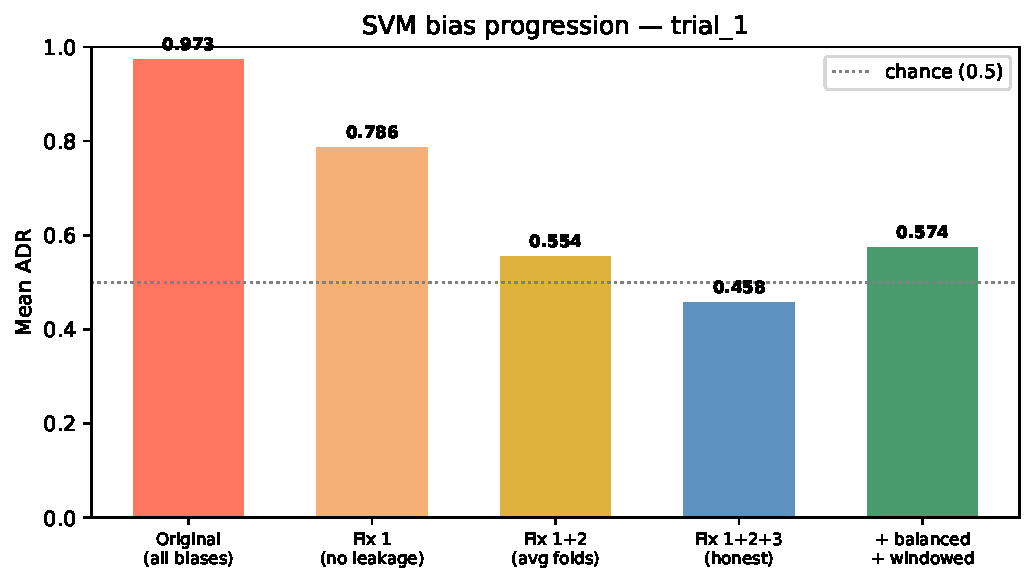
\includegraphics[width=\columnwidth]{figures/fig_bias_progression}
  \caption{SVM ADR across pipeline variants (trial\_1). Each correction removes one source of optimistic assumption; the rightmost bar is the revised baseline.}
  \label{fig:bias_progression}
\end{figure}

\subsection{Initial DL Evaluation (5 Seeds)}

Table~\ref{tab:dl_results} reports ADR for each DL model under a group-aware
70/15/15 split, averaged over five random seeds (trial\_1). All three models
achieve ADR between 0.62 and 0.68.

\begin{table}[htbp]
\centering
\caption{DL model ADR on held-out test set (trial\_1, 5 seeds).}
\label{tab:dl_results}
\begin{tabular}{lc}
\toprule
\textbf{Model} & \textbf{ADR (mean $\pm$ std)} \\
\midrule
MLP-FV            & \mlpADR \\
GRU-DGT           & \gruADR \\
BiGRU+TF-Aug & \bigruADR \\
\bottomrule
\end{tabular}
\end{table}

\begin{figure}[htbp]
  \centering
  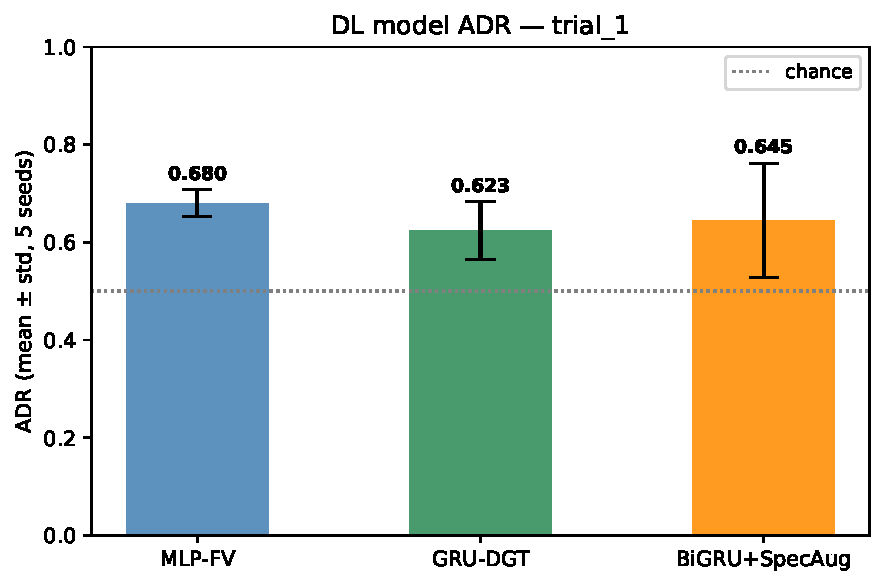
\includegraphics[width=\columnwidth]{figures/fig_dl_adr}
  \caption{DL model ADR (mean $\pm$ std, 5 seeds, trial\_1). The wide error bar on BiGRU signals that five seeds are insufficient for reliable conclusions.}
  \label{fig:dl_adr}
\end{figure}

The BiGRU in particular exhibits high variance (seed ADR range \bigruSeedADRMin--\bigruSeedADRMax). With only
$n=5$ seeds the confidence intervals are too wide to draw reliable conclusions
about relative model performance. This motivated adopting LOTO cross-validation as the primary evaluation protocol, maximising use of the limited dataset.

\subsection{LOTO Cross-Validation (Primary Evaluation)}

LOTO (Leave-One-Transient-Out) holds out one complete transient per fold, making use of every available sample while remaining strictly transient-aware. Table~\ref{tab:loto} reports per-device ADR and EER for the BiGRU on trial\_1. Mean ADR is \bigruLOTOadrMean{} and mean EER is \bigruLOTOeerMean{}, well above the chance EER of 0.5, confirming above-chance device discrimination across all authorized devices.

\begin{table}[htbp]
\centering
\caption{BiGRU LOTO per-device ADR and EER (trial\_1).}
\label{tab:loto}
\begin{tabular}{lcc}
\toprule
\textbf{Device} & \textbf{ADR} & \textbf{EER} \\
\midrule
device2  & \bigruLOTOadrTwo   & \lotoEERTwo \\
device3  & \bigruLOTOadrThree & \lotoEERThree \\
device9  & \bigruLOTOadrNine  & \lotoEERNine \\
device12 & \bigruLOTOadrTwelve & \lotoEERTwelve \\
\midrule
\textbf{Mean} & \textbf{\bigruLOTOadrMean} & \textbf{\bigruLOTOeerMean} \\
\bottomrule
\end{tabular}
\end{table}

\begin{figure}[htbp]
  \centering
  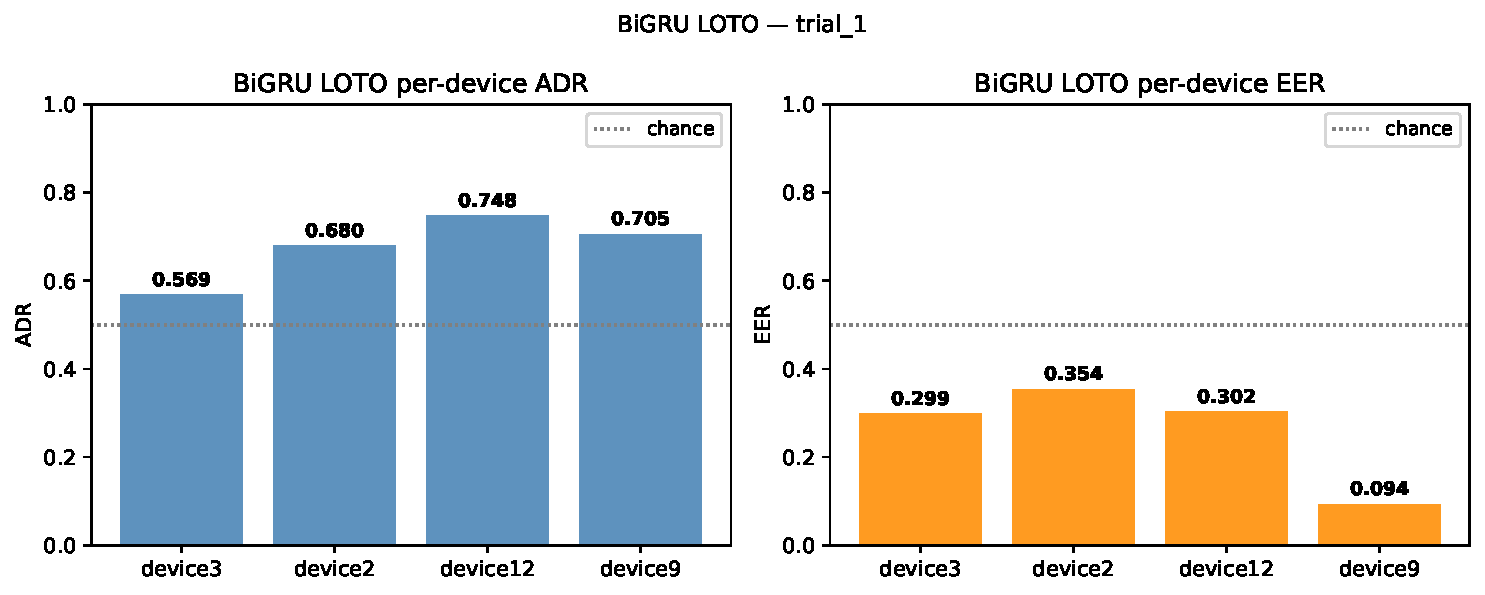
\includegraphics[width=\columnwidth]{figures/fig_loto_eer}
  \caption{BiGRU LOTO per-device ADR and EER (trial\_1). Dashed line marks chance level (EER~$= 0.5$).}
  \label{fig:loto_eer}
\end{figure}

\subsection{ML vs.\ DL Comparison}

Fig.~\ref{fig:ml_vs_dl_loto} places the revised SVM alongside all three DL models
evaluated under LOTO cross-validation. No pipeline has a clear advantage: all models
cluster in a \svmADR--\bigruLOTOadrMean{} ADR band with overlapping uncertainty. The performance gap
between the original and revised pipelines is entirely attributable to evaluation
methodology.

\begin{figure}[htbp]
  \centering
  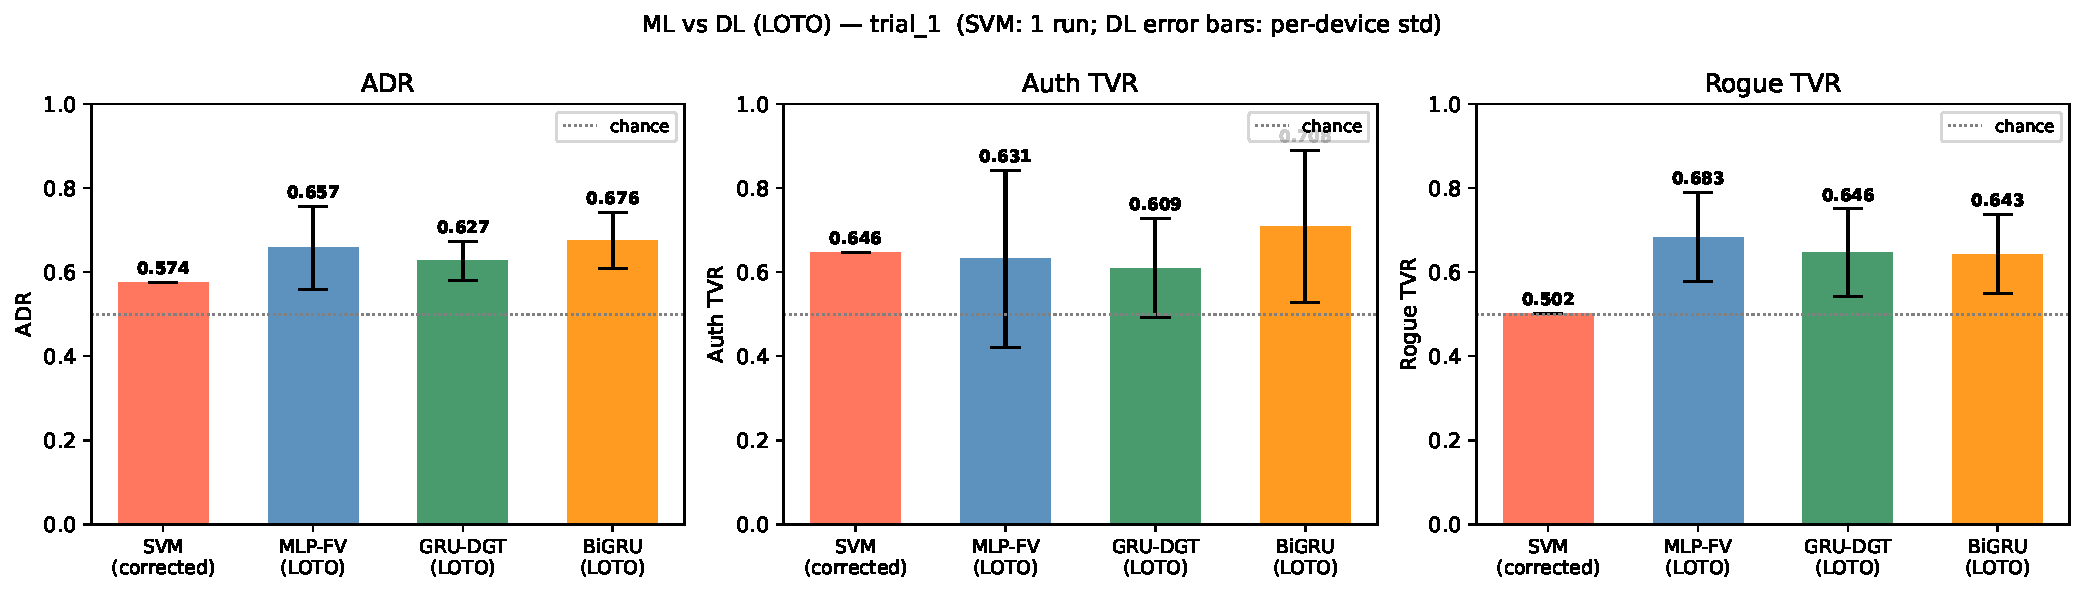
\includegraphics[width=\columnwidth]{figures/fig_ml_vs_dl_loto}
  \caption{ML vs.\ DL (LOTO): ADR, Auth TVR, and Rogue TVR (trial\_1).
           SVM error bar is zero (single deterministic run);
           DL bars are $\pm$1 std across authorized devices (LOTO).}
  \label{fig:ml_vs_dl_loto}
\end{figure}


\section{Summary and Contributions}
\label{sec:contributions}
\subsection*{What We Found}
\begin{itemize}
  \item The original RF-DNA SVM pipeline contains three independent evaluation biases that collectively inflate reported ADR from $\svmOrigADR \to \svmADR$ (approximately 40 percentage points).
  \item Under a fair evaluation protocol, SVM and all three DL models
        (MLP-FV, GRU-DGT, BiGRU+TF-Aug) achieve statistically equivalent ADR in the 0.57--0.68 range. No architecture is a clear winner.
  \item With only five seeds the BiGRU shows ADR variance of $\pm 0.131$;
        LOTO cross-validation provides more stable per-device estimates
        (mean ADR \bigruLOTOadrMean, mean EER \bigruLOTOeerMean).
  \item Dataset size is the primary performance bottleneck: each binary
        classifier in trial\_1 trains on $\approx$52 windowed samples,
        far below what DL models typically require to generalise reliably.
\end{itemize}

\subsection*{Contributions}
\begin{itemize}
  \item \textbf{Revised baseline.} Identified, isolated, and quantified three evaluation assumptions in the original RF-DNA pipeline, providing reproducible corrections with per-bias ADR measurements.
  \item \textbf{Honest DL baseline.} First evaluation of MLP, GRU, and BiGRU architectures on this dataset under a strictly group-aware, transient-aware protocol across five seeds and LOTO.
  \item \textbf{Data-efficiency result.} Demonstrated that sliding-window augmentation enables DL training with 10$\times$ fewer recordings by exploiting the full transient duration, confirming that device-discriminating hardware imperfections persist well beyond the initial signal segment used by the original pipeline.
  \item \textbf{Multi-class probe.} Showed that a single BiGRU trained on all 12 devices reaches \mcAccuracy{} accuracy (vs.\ \mcRandomBaseline{} random), confirming that discriminative information exists across all devices and that architecture is not the limiting factor while dataset size is (Appendix~\ref{app:multiclass}).
\end{itemize}

\subsection*{Future Directions}
\begin{itemize}
  \item Collect additional independent transients per device to push ADR toward
        operationally useful levels.
  \item Evaluate AND-aggregation at system level to reduce the high False Accept
        Rate under OR-aggregation.
  \item Explore per-device classifier ensembles: training multiple models per
        authorized device and combining their outputs via soft voting could
        reduce the high seed-to-seed variance observed in this work and yield
        more stable authentication decisions without architectural changes.
  \item Conduct adversarial robustness evaluation (white-box and black-box
        attacks on raw IQ waveforms), now that an honest unattacked baseline
        is established.
\end{itemize}


\section{Conclusion}
\label{sec:conclusion}
This report established a rigorous, reproducible performance baseline for RF
fingerprinting on a 12-device dataset. A complete DL pipeline was evaluated under a rigorous, group-aware protocol;
all models achieve ADR in the 0.57--0.68 range,
confirming that RF transient emissions carry sufficient device-discriminating
information to support PLA above chance, while highlighting per-classifier
sample count as the binding constraint. Addressing this --- through larger
datasets or improved augmentation strategies --- is the most direct path
toward operationally useful PLA. Future directions are listed in
Section~\ref{sec:contributions}.

Two results have direct implications for practical deployment. First, the
high seed-to-seed variance of the BiGRU ($\Delta$ADR up to 0.37 across seeds
for a single trial) means the system is not yet reliable enough for deployment
at fixed thresholds; an ensemble or calibration step is needed before
per-device classifiers can operate at a stable operating point. Second, the
multi-class probe --- which achieves substantially higher relative gain over
chance despite identical data --- suggests that joint training across all
devices is the right inductive bias for a dataset of this size, and warrants
prioritisation over further tuning of per-device binary classifiers.


\newpage

\appendix

\section{RnF+ANOVA Protocol Variants}
\label{app:rnf_variants}
Fig.~\ref{fig:bias_progression} shows the ADR progression across the four
RnF pipeline protocol variants for trial\_1. The original pipeline reports
near-perfect ADR under the paper protocol; each successive variant applies one
additional deployment constraint, yielding ADR~$\approx 0.574$ under the full
deployment-condition baseline for trial\_1.

\begin{figure}[htbp]
  \centering
  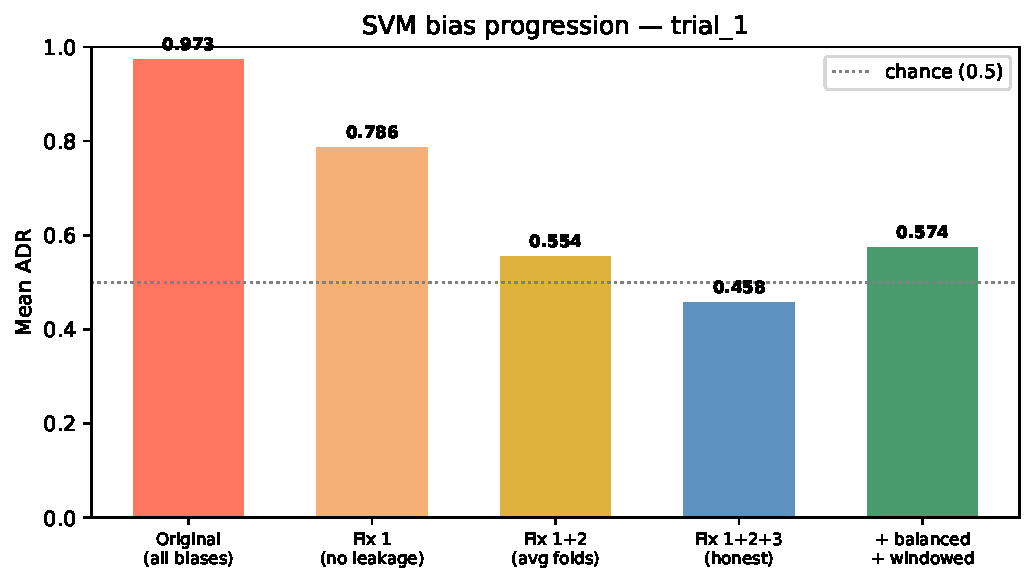
\includegraphics[width=\columnwidth]{figures/fig_bias_progression}
  \caption{RnF+ANOVA ADR across protocol variants (trial\_1). The rightmost column shows the effect of windowed augmentation on the Variant~A+B+C pipeline.}
  \label{fig:bias_progression_app}
\end{figure}
These results confirm that the signal contains device-discriminating information; all devices achieve ADR above the chance level of 0.5.


\section{Multi-class Feasibility Probe}
\label{app:multiclass}
To test whether the binary per-device setup is the binding constraint,
a single BiGRU + TF-Aug is trained on all 12 devices simultaneously
(12-class softmax). The model has access to the full \nWindowedSamples-sample windowed
DGT cache, compared to the $\approx$52 samples available to each binary
classifier in trial\_1.

\begin{table}[htbp]
\centering
\caption{Multi-class BiGRU vs.\ binary LOTO (trial\_1, 5 seeds).}
\label{tab:multiclass}
\begin{tabular}{lcc}
\toprule
\textbf{Setting} & \textbf{Metric} & \textbf{Value} \\
\midrule
Binary LOTO (BiGRU)    & mean ADR  & \bigruLOTOadrMean \\
Multi-class (BiGRU)    & accuracy  & $\mcAccuracy \pm \mcAccuracyStd$ \\
Multi-class (BiGRU)    & macro F1  & $\mcMacroFone \pm \mcMacroFoneStd$ \\
Random baseline (1/12) & accuracy  & \mcRandomBaseline \\
\bottomrule
\end{tabular}
\end{table}

% figures/fig_mc_confusion and fig_mc_perclass not yet generated (run notebook 04 export cell)
%\begin{figure}[htbp]
%  \centering
%  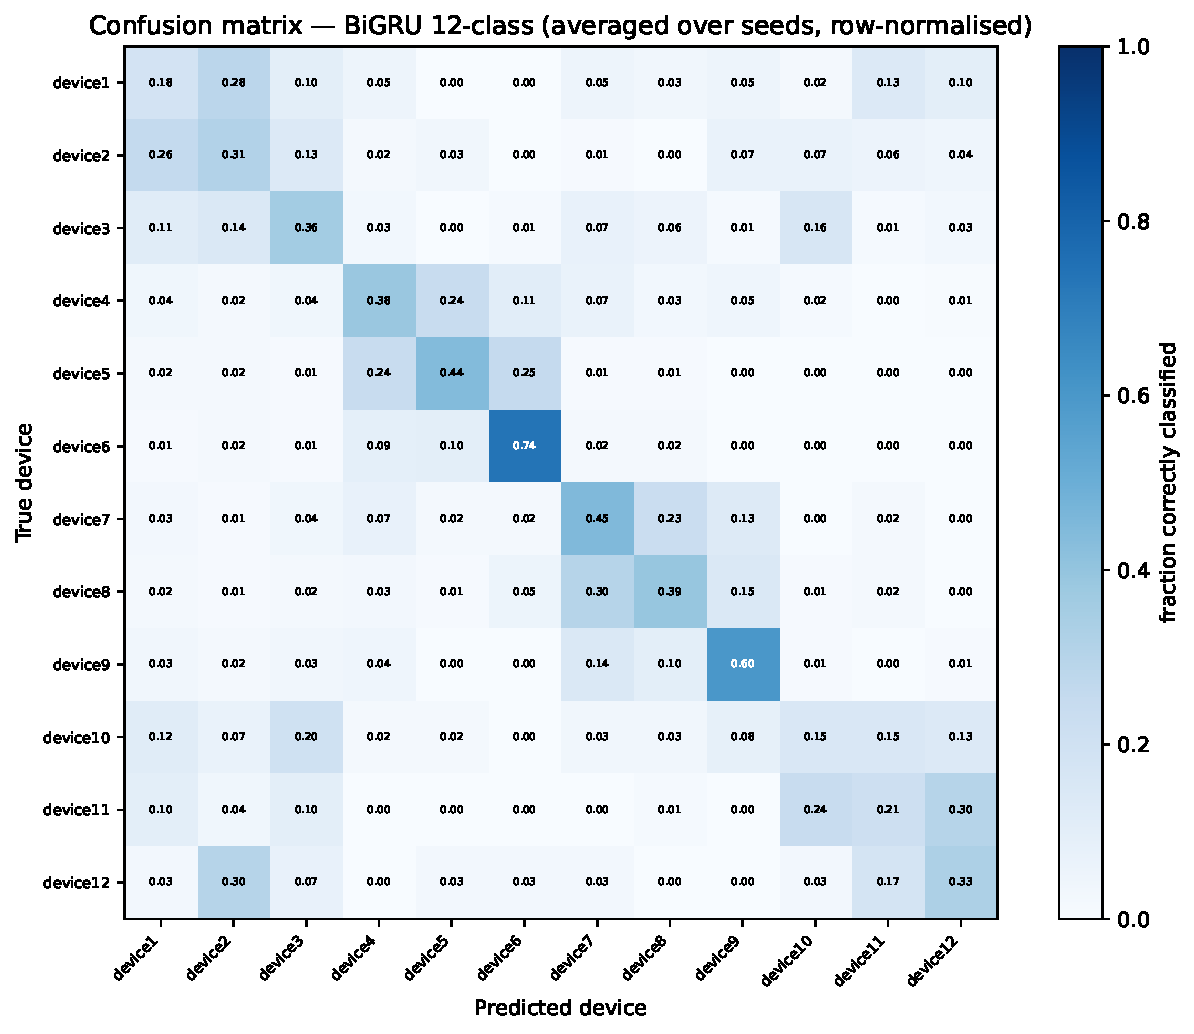
\includegraphics[width=\columnwidth]{figures/fig_mc_confusion}
%  \caption{Averaged confusion matrix (BiGRU, 12-class, 5 seeds).
%           Row-normalised; diagonal dominance indicates above-chance discrimination.}
%  \label{fig:mc_confusion}
%\end{figure}
%
%\begin{figure}[htbp]
%  \centering
%  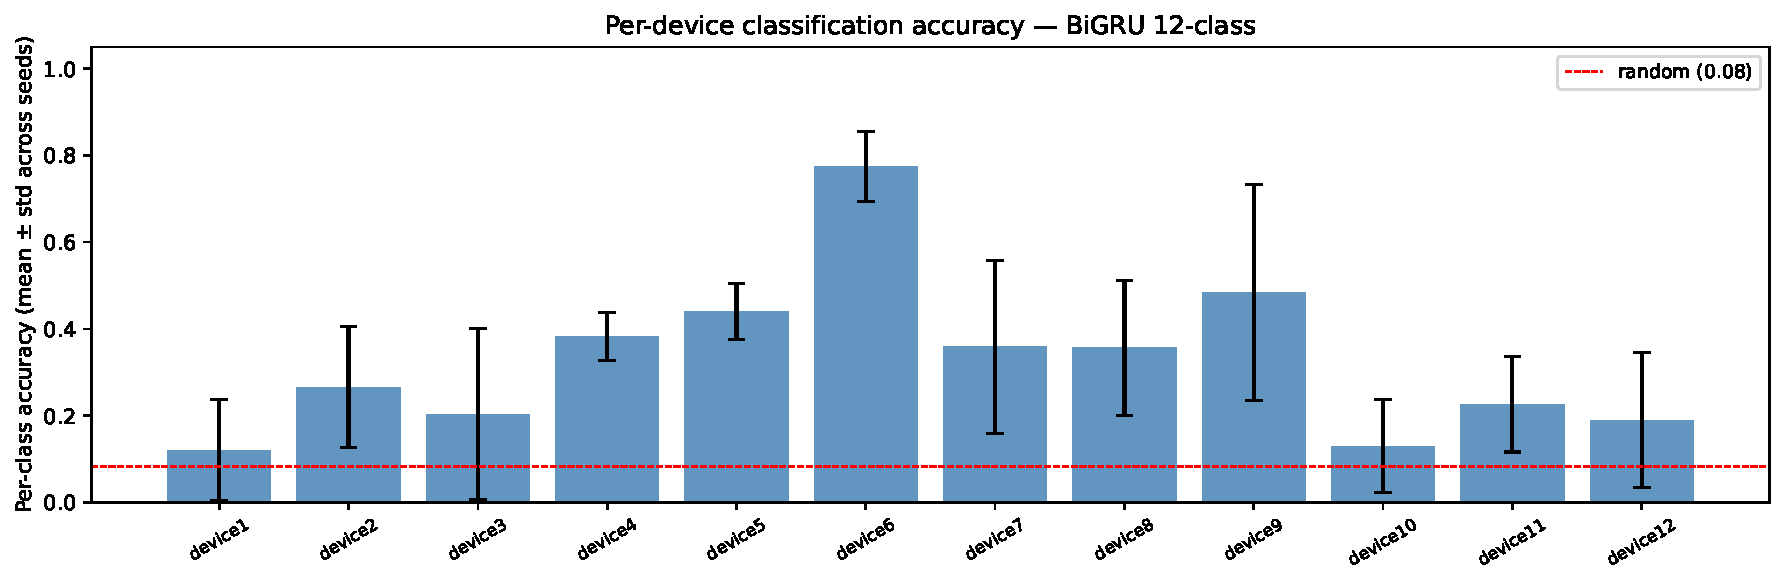
\includegraphics[width=\columnwidth]{figures/fig_mc_perclass}
%  \caption{Per-device classification accuracy (mean $\pm$ std, 5 seeds).
%           Devices with fewer raw transients (device10--12) show higher variance.}
%  \label{fig:mc_perclass}
%\end{figure}

The multi-class BiGRU achieves \mcAccuracy\% accuracy against a random baseline of
\mcRandomBaseline, confirming that the RF transient carries device-discriminating information across all 12 devices. In absolute terms this is lower than the binary LOTO ADR (\bigruLOTOadrMean), which reflects the harder 12-way classification task rather than a failure of the architecture. Devices 10--12, which have only 60 windowed samples each compared to 120--130 for devices 1--9, display the highest variance, reinforcing that per-device sample count is the primary performance driver.


\section{Extended Discussion}
\label{app:discussion}
% ── 0. Scope of the revised audit ───────────────────────────────────────────────
\subsection{Scope of the Pipeline Evaluation: Why RnF+ANOVA}

The ML analysis in this work is deliberately scoped to the original
RF-DNA pipeline from \texttt{RF\_Fingerprint.py}: a Random Forest
(n\_estimators=10, max\_depth=8) preceded by ANOVA-based feature selection (\texttt{SelectKBest} with
the F-test statistic).
This is not the only possible ML pipeline for the 505-dimensional feature
vector. In fact the same code base also implements mutual information, RFE, and PCA as alternative selectors, and other classifiers such as SVM or
$k$-NN could in principle be substituted.


\textbf{Time constraints.}
Extending the evaluation to alternative classifiers and feature selectors
was outside the scope of this project.
Each additional pipeline variant requires its own replication, its own
characterisation, and its own aligned baseline.
Given the available time, the decision was to perform a thorough audit of
the single pipeline that was actually used, rather than a shallow
survey of many alternatives.

% ── 1. Feasibility confirmed — but at what operating point? ──────────────────
\subsection{Feasibility Confirmed, but Operationally Insufficient}

All pipelines achieve ADR consistently above the chance level of 0.5,
which confirms the central premise of RF fingerprinting: hardware
imperfections embedded in power-on transients are statistically
discriminable by both classical and deep models.
However, the gap between feasibility and operational deployment deserves
careful framing.

% ── 2. MLP-FV vs BiGRU: a result that depends on the evaluation ──────────────
\subsection{MLP-FV vs.\ BiGRU: Results Depend on the Evaluation Protocol}

Comparing MLP-FV and BiGRU+TF-Aug requires reading both evaluations
together, because the two protocols give different orderings.

In the \emph{simple held-out evaluation} (one fixed 70/15/15 split per seed,
five seeds), MLP-FV achieves a higher mean ADR (\mlpADR) than
BiGRU+TF-Aug (\bigruADR).
However, BiGRU's per-seed ADRs span from \bigruSeedADRMin{} to \bigruSeedADRMax{} --- a range of \bigruSeedADRRange{}
across just five runs --- while MLP's range is only \mlpSeedADRRange{} (\mlpSeedADRMin--\mlpSeedADRMax).
With such wide and overlapping confidence intervals ($n=5$), the difference in means is \emph{not statistically significant}.
The higher mean of MLP in this evaluation is better explained by the fact that one BiGRU seed collapsed to ADR~$=0.471$ (below chance for rogue TVR) while another peaked at ADR~$=0.838$, averaging to a moderate figure that happens to fall below MLP's stable mean.

Under \emph{LOTO cross-validation} --- the more data-efficient and arguably
more rigorous protocol, the ordering reverses:
BiGRU achieves mean ADR~$=\bigruLOTOadrMean$, MLP achieves $\mlpLOTOadrMean$, and GRU achieves
$\gruLOTOadrMean$.
LOTO removes the threshold-variability issue (each fold calibrates its own threshold) and maximises training data, providing a more stable comparison surface.
On this evidence, BiGRU is marginally better than MLP, not worse.

A structural reason why MLP-FV performs similarly to BiGRU is that its 505-dimensional feature vector is the result of deliberate
domain engineering that distinguishes hardware imperfections.
An MLP operating on this input does not need to learn which features matter
because the engineering has done that; a BiGRU on raw DGT must discover
the same information from scratch.

The practical implication is that the RF-DNA feature vector is not merely a legacy artefact: its domain-engineered statistics act as a built-in dimensionality reduction and noise suppression layer that compensates for the limited training set. This could serve as an intermediate representation within a deeper DL pipeline by pre-processing the signal into a compact, domain-informed descriptor and then feeding it to a more expressive classifier. This hybrid strategy could inherit the stability advantages of hand-crafted features while retaining the capacity to learn higher-level discriminative patterns, making it particularly well-suited to small-dataset RF fingerprinting regimes.

% ── 5. Validation-based threshold calibration ────────────────────────────────
\subsection{Validation-Based Threshold Calibration: Tried and Rejected}

A natural question when reporting LOTO results is whether the fixed decision threshold of 0.5 is optimal, or whether it can be improved by selecting the threshold from the available validation data. The LOTO pipeline was instrumented to answer this: after all folds complete, the validation scores from every fold are pooled per device and the threshold that maximises ADR on that pooled validation set is found via the ROC curve. This val-optimal threshold is then applied to the pooled test scores, giving a second set of results alongside the fixed-threshold results.

Table~\ref{tab:threshold_cal} shows the outcome for the BiGRU on trial\_1.

\begin{table}[htbp]
\centering
\caption{BiGRU LOTO: ADR at fixed threshold (0.5) vs.\ val-calibrated threshold (trial\_1).}
\label{tab:threshold_cal}
\begin{tabular}{lccc}
\toprule
\textbf{Device} & \textbf{ADR @ 0.5} & \textbf{ADR @ opt} & \textbf{Opt threshold} \\
\midrule
device2  & \bigruLOTOadrTwo   & \bigruLOTOadrOptTwo   & \bigruLOTOthrTwo \\
device3  & \bigruLOTOadrThree & \bigruLOTOadrOptThree & \bigruLOTOthrThree \\
device9  & \bigruLOTOadrNine  & \bigruLOTOadrOptNine  & \bigruLOTOthrNine \\
device12 & \bigruLOTOadrTwelve & \bigruLOTOadrOptTwelve & \bigruLOTOthrTwelve \\
\midrule
\textbf{Mean} & \textbf{\bigruLOTOadrMean} & \textbf{\bigruLOTOadrOptMean} & — \\
\bottomrule
\end{tabular}
\end{table}

Val-calibration \emph{hurts} overall: mean ADR drops from \bigruLOTOadrMean{} to \bigruLOTOadrOptMean.
The same pattern holds for MLP-FV (\mlpLOTOadrMean~$\to$~\mlpLOTOadrOptMean) and GRU-DGT
(\gruLOTOadrMean~$\to$~\gruLOTOadrOptMean). The root cause is visible in the device12 row.

This is a direct consequence of the validation set being too small to reliably
estimate a good threshold. Device12 has only 6 transients total; after
reserving one as the test fold and one for early stopping per fold, the pooled
val scores across all folds are too few and too concentrated to produce a
stable operating point.

The practical conclusion is clear: \textbf{with this dataset size, the default
threshold of 0.5 is more robust than any data-driven alternative}. Threshold
calibration becomes worthwhile only when the calibration set is large enough to
produce a smooth, representative score distribution...a condition this dataset
does not meet.

% ── 6. Multi-class probe reinterpreted ───────────────────────────────────────
\subsection{Multi-class Accuracy Reinterpreted}

At first glance, the multi-class BiGRU accuracy of $0.404 \pm 0.057$ appears
lower than the binary LOTO ADR of 0.676, suggesting the multi-class model
performs worse.
This comparison is misleading because the two tasks differ fundamentally.

In binary LOTO, the model answers a yes/no question for one device against
8 rogues, with a balanced or threshold-corrected decision boundary.
In multi-class, the model must identify the correct one among 12 devices.
The appropriate reference is not 0.5 (binary chance) but $1/12 \approx 0.083$
(multi-class chance).
Measured as relative improvement over the random baseline:
\begin{align}
  \text{Binary LOTO gain} &= \frac{\bigruLOTOadrMean - 0.500}{0.500} = \binaryLOTORelGain\%,\\
  \text{Multi-class gain} &= \frac{\mcAccuracy - \mcRandomBaseline}{\mcRandomBaseline} = \mcRelGain\%.
\end{align}
By this normalised measure, the multi-class model demonstrates \emph{more}
discriminative power, not less.


% ── 8. Representational limits ───────────────────────────────────────────────
\subsection{Representational Limits of the DGT Approach}

The current pipeline extracts features from a single power-on transient.
This is a one-time event spanning roughly 100\,000 samples ($\approx$5\,ms
at 20\,MHz): once the power-on transient ends, this fingerprinting opportunity
is gone until the next power cycle.
In real network scenarios, devices remain active for extended periods.
The transient-only approach would require re-authentication at each
power-cycle, which limits applicability in continuously running networks.

An alternative that has not been explored here is \emph{steady-state
fingerprinting}: exploiting clock imperfections, carrier frequency offset,
or I/Q imbalance from normal data frames.
Steady-state features can be extracted from any 802.11 packet, enabling
continuous authentication without requiring special transient events.
Combining transient and steady-state features would likely improve both
accuracy and coverage.

Additionally, the DGT matrix of size 150$\times$150 is large relative to
the information it encodes per transient.
Much of the matrix may be occupied by noise or uninformative regions.
An attention mechanism (Transformer self-attention on the row sequence, or
a spatial attention map over the 2D matrix) could learn to focus on the
discriminative regions automatically, rather than requiring the entire
matrix to be processed at equal cost.

% ── 9. Missing experiments and open questions ─────────────────────────────────
\subsection{Missing Experiments and Open Questions}

Several experiments that would substantially strengthen the conclusions
were not performed, either due to dataset constraints or scope limitations.

\textbf{TF-Aug ablation.}
As discussed above, the contribution of time-frequency masking augmentation to BiGRU performance
is unknown because no BiGRU-without-TF-Aug baseline was recorded.

\textbf{2D convolutional baseline.}
The GRU/BiGRU models impose a sequential scan over a 2D DGT matrix.
A CNN applied to the same matrix as a 2D image
would test whether the performance floor is architectural (sequential
models are wrong for this data) or purely dataset-size related.

\textbf{Adversarial evaluation.}
The original goal of the project was adversarial robustness evaluation.
Now that a baseline exists, there could be a tractable attack direction.

\textbf{Larger dataset evaluation.}
The most direct path to operational ADR is more data. This projection is speculative but motivates a data collection campaign as the first step toward a practical PLA system.

\subsubsection*{Which approach is more appropriate for this task?}

Neither approach is clearly superior given the current dataset size.
The RnF is more data-efficient and produces stable, reproducible results
because it does not have random weight initialisation.
However, its decision boundary in a fixed feature space is a
fundamental capacity limit that cannot be overcome by adding more data.

Deep learning has no such architectural ceiling: given enough data,
deeper or more complex architectures can fit arbitrarily complex decision
boundaries.
The multi-class probe already shows that the BiGRU, given access to 25$\times$
more samples (1340 vs.\ 52), achieves a relative improvement over random
chance that is $11\times$ larger than the binary RnF classifier.
This strongly suggests that deep learning is the right long-term direction,
but that the current dataset does not yet have enough examples to let deep
models demonstrate their advantage.

\bibliographystyle{IEEEtran}
\bibliography{references}

\EOD

\end{document}
